%________________________________________________________
\section{Flow of the analysis procedure}
\label{Note:FLOW}

Fig.\,\ref{Note:FigAnalysisFlow} shows a schematic view of the flow of the analysis procedure. The first thing a typical user needs to do in order to analyze events stored on the GRID, is to interact with the file catalog in order to define the collection of files that he/she needs. This action implies the usage of the metadata fields assigned at the level of a run. Detailed description about the structure of the file catalog as well as the metadata fields on this level can be found in \cite{Note:RefFileCatalogMetadataNote,Note:RefFileCatalogMetadataWeb}. As an example, we have a user that wants to create a collection of tag files that fulfill the following criteria:

\begin{itemize}
\item The production year should be 2008.
\item The period of the LHC machine should be the first of 2008.
\item The data should come from the third reconstruction pass.
\item The collision system should be p+p.
\item The start and stop time of the run should be beyond the 19th of March 2008 and no later than 10:20 of the 20th of March 2008 respectively.
\end{itemize}

\noindent Then what needs to be written in the AliEn shell \cite{Note:RefFileCatalogMetadataWeb} (as a one line command) is:

\begin{lstlisting}[language=sh]
  find -x pp /alice/data/2008/LHC08a/*/reco/Pass3/* *tag.root 
  Run:collision_system=''pp'' and Run:stop<''2008-03-20 10:20:33'' 
  and Run:start>''2008-03-19'' > pp.xml
\end{lstlisting}

The previous lines imply the use of the {\ttfamily find} command of the alien shell \cite{Note:RefAlienTutorial}. The first argument of this command is the name of the collection which will be written inside the file. If the {\ttfamily -x pp} option is not used then we will not get back all the information about the file but instead we will just retrieve the list of logical file names (lfn). Then comes the path of the file catalog under which the files we want to analyze are stored followed by the name of the file. In this example, the path implies that the user requests a collection of real data ({\ttfamily /alice/data}) coming from the first period of the LHC machine in year 2008 ({\ttfamily /2008/LHC08a}), containing all the run numbers of the third pass of the reconstructed sample ({\ttfamily /*/reco/Pass3}). The last argument is the metadata fields: a variety of such fields can be combined using logical statements. The reader should notice that the output of this command is redirected to a xml file, which consists of all the necessary information (the file's unique identifier - guid, the logical file name etc) about the files that fulfill the imposed selection criteria. This xml collection, which is stored in the local and not the Grid working directory,  plays a very important role in the overall distributed analysis framework as we will see in the next sections. From the above example it is obvious that wild cards can be used.

Going back to the description of Fig.\,\ref{Note:FigAnalysisFlow} and following the flow of the arrows, we assume that the user creates a tag xml collection. Then in parallel inside a macro he/she imposes some selection criteria at the event level. Having those two components as an input, the \tag\ is queried and from this action, the system can either provide directly the input data collection, which is a chain of ESD files along with the associated event list (which describes the events that fulfill the imposed selection criteria), or a new ESD xml \footnote{This is different to the tag xml collection discussed earlier.} collection (mainly used for batch analysis --- see section \ref{Note:BATCH} for details). Even in the latter case, we end up having the chain along with the associated event list. This chain can then be processed by an analysis manager \cite{Note:RefAnalysisFramework} either locally, in AliEn \cite{Note:RefALIEN}, or using PROOF \cite{Note:RefPROOF}.

\begin{figure}[ht!]
\begin{center}
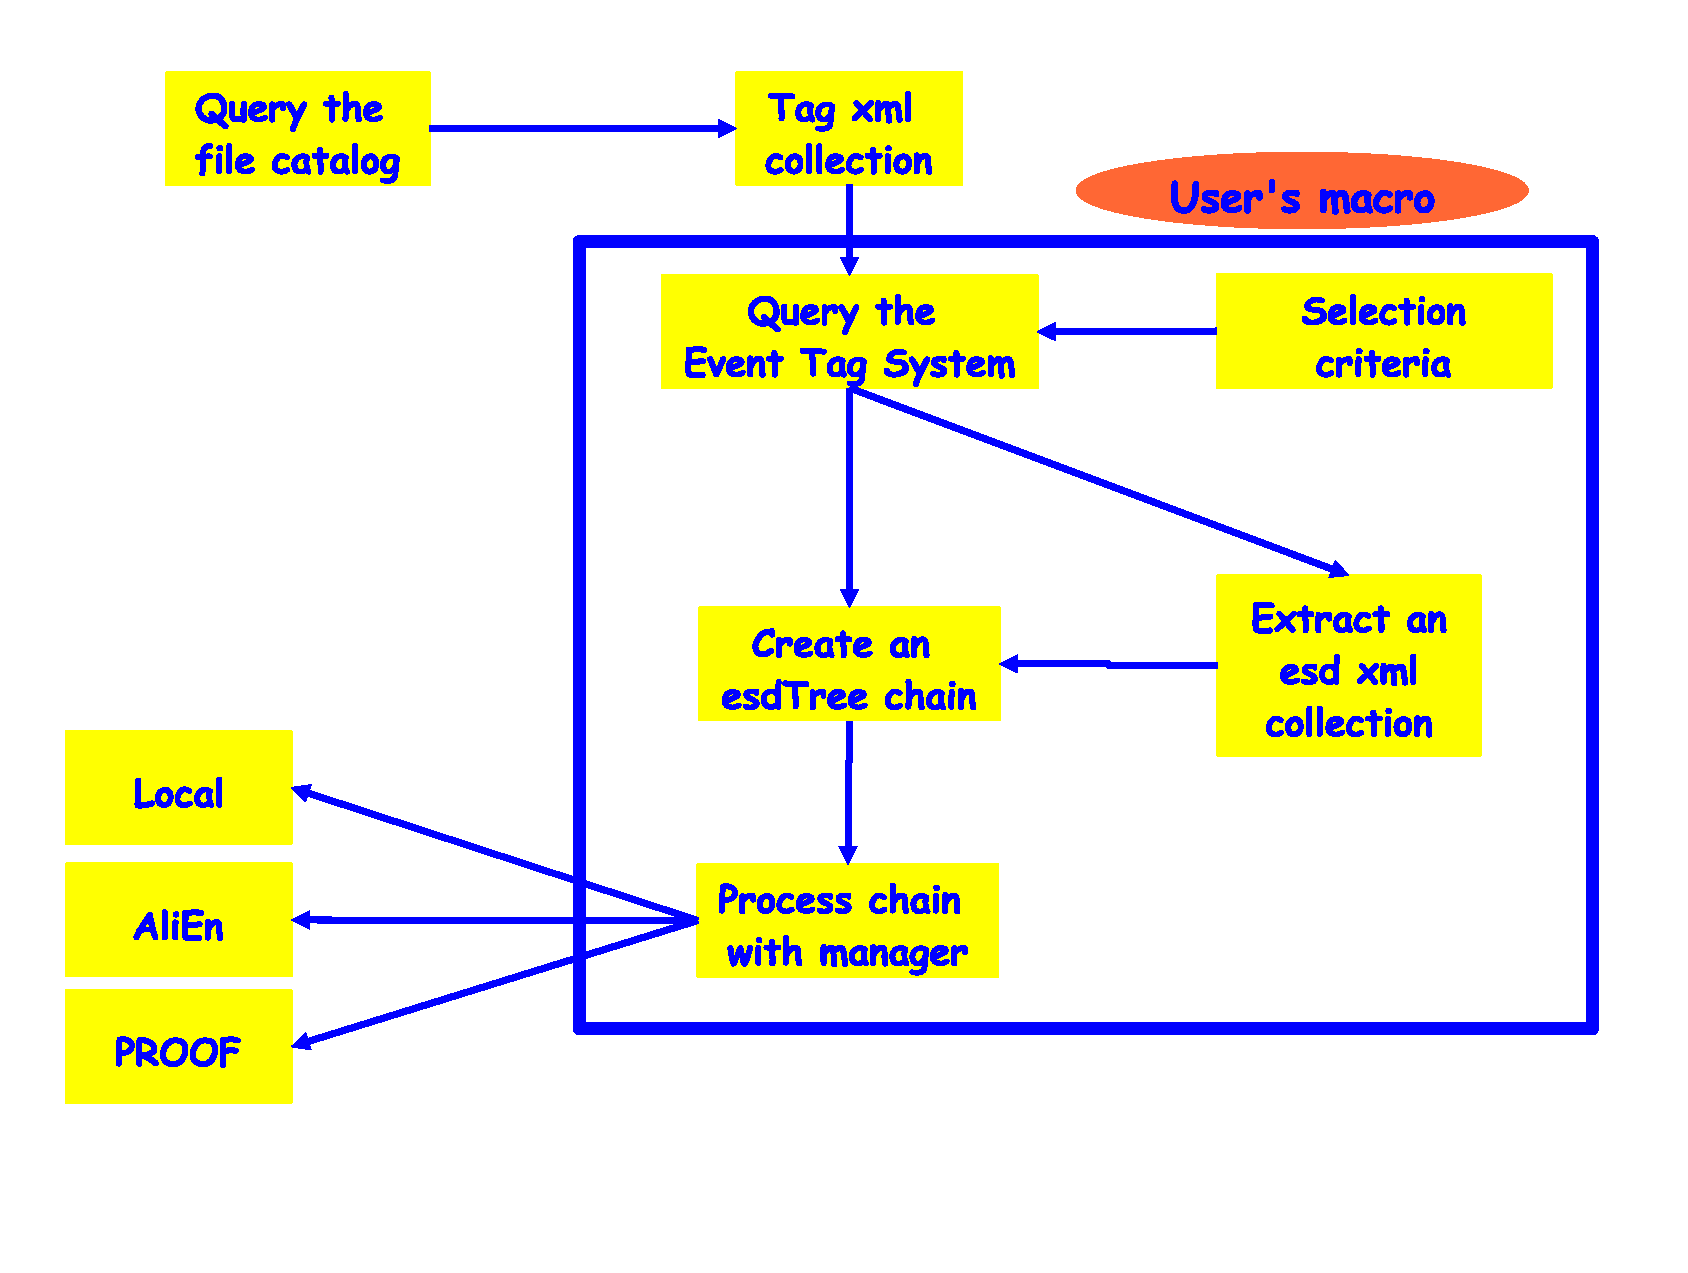
\includegraphics[width=0.7\textheight]{figures/Flow.eps}
\end{center}
\caption{The flow of the analysis procedure: Having as an input the tag xml collection that we create by querying the file catalog and the selection criteria, we interact with the \tag\ and we either get a chain along with the associated event list (events that fulfill the imposed selection criteria) or we create an ESD xml collection (for batch sessions) from which we create the ESD chain. This chain is processed with an analysis manager locally, in AliEn or even in PROOF.}
\label{Note:FigAnalysisFlow}
\end{figure}

We would also like to point out that we have two options on how to use the framework:

\begin{itemize}
\item We can work with aliroot and try all the examples that will be described in the next sections by loading all the corresponding libraries.
\item We can try to be as flexible as possible, by running ROOT along with the corresponding aliroot libraries (e.g. in the case of the analysis of AliESDs.root we need just the libESD.so along with the libANALYSIS\_NEW.so - the latter is needed for the new analysis framework which will be described in the next section). These libraries are created from the compilation of the relevant aliroot code which can be included in the so called {\ttfamily par file}. This par file is nothing more than a tarball containing the .h and .cxx aliroot code along with the Makefile and Makefile.arch (needed to compile the aliroot code in different platforms).
\end{itemize}

The user has these two possibilities although for some cases, like the analysis of generator information, the second option can't be used: we need to launch aliroot. In the following examples we will always concentrate in the case where we use the {\ttfamily par file}. The lines listed below show how we can setup, compile and load the libESD.so from the {\ttfamily ESD.par}.

\vspace{2 cm}

\begin{lstlisting}[language=C++]
  const char* pararchivename = "ESD";
  // Setup PAR File
  if (pararchivename) {
    char processline[1024];
    sprintf(processline,".! tar xvzf %s.par",pararchivename);
    gROOT->ProcessLine(processline);
    const char* ocwd = gSystem->WorkingDirectory();
    gSystem->ChangeDirectory(pararchivename);

    // check for BUILD.sh and execute
    if (!gSystem->AccessPathName("PROOF-INF/BUILD.sh")) {
      printf("*******************************\n");
      printf("*** Building PAR archive    ***\n");
      printf("*******************************\n");

      if (gSystem->Exec("PROOF-INF/BUILD.sh")) {
        Error("runProcess","Cannot Build the PAR Archive! - Abort!");
        return -1;
      }
    }
    // check for SETUP.C and execute
    if (!gSystem->AccessPathName("PROOF-INF/SETUP.C")) {
      printf("*******************************\n");
      printf("*** Setup PAR archive       ***\n");
      printf("*******************************\n");
      gROOT->Macro("PROOF-INF/SETUP.C");
    }
    
    gSystem->ChangeDirectory("../");
  }
  gSystem->Load("libVMC.so");
  gSystem->Load("libESD.so");
\end{lstlisting}

